\section{Kort introduktion till programmering i \coq och utvecklingsmiljön \coq
Ide}

\subsection{Beskrivning av \coq Ide}


% Förtext till bild. Nämn figur

\begin{enumerate}
\item Textredigerare. I den här rutan skriver användaren sina program och bevis
\item Textfönster för mål och kontext. Här visas vilka mål man vill uppnå och
  vilka värden man för närvarande har i kontext. Dessa uppdateras efter varje
  utförd taktik.
\item Textfönster för meddelanden. Här dyker felmeddelanden, svar på
  gjorda sökningar och övrig information upp.
\item Symboler för att stega framåt eller bakåt i koden. När vi stegar framåt
  evalueras koden som stegas förbi.
\end{enumerate}

\begin{figure}[H]
  \centering
  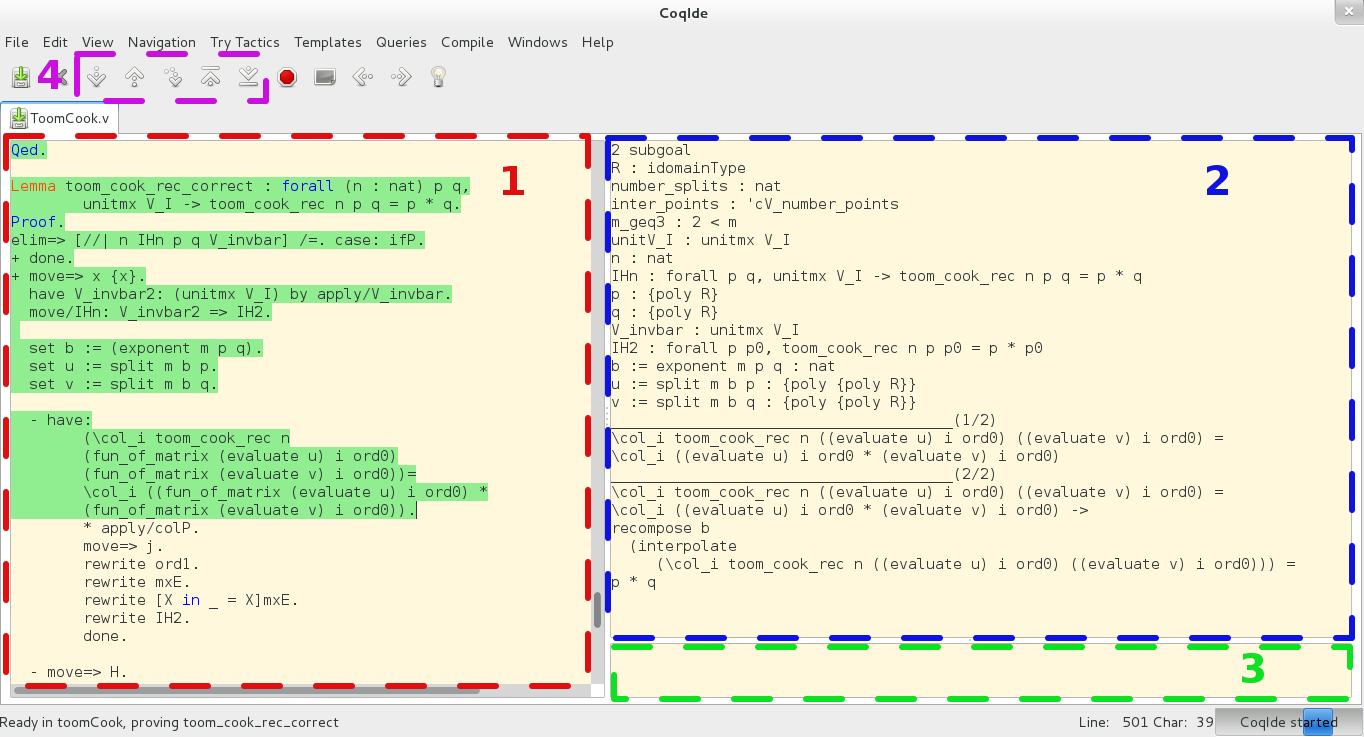
\includegraphics[width=\textwidth]{images/Overview}
  \caption[Översikt av \coq Ide]
   {Översikt av de olika delarna i \coq Ide}
\end{figure}

\begin{enumerate} % börja på 5
\item Kontext, här visas vilka hypoteser och variabler som vi för tillfället
  har i beviset.
\item Mål, här visas vilka mål som ska uppnås. Det översta målet är det som
  användaren arbetar med för tillfället och det är det målet som kommer att
  påverkas av nästkommande taktik.
\end{enumerate}

\begin{figure}[H]
  \centering
  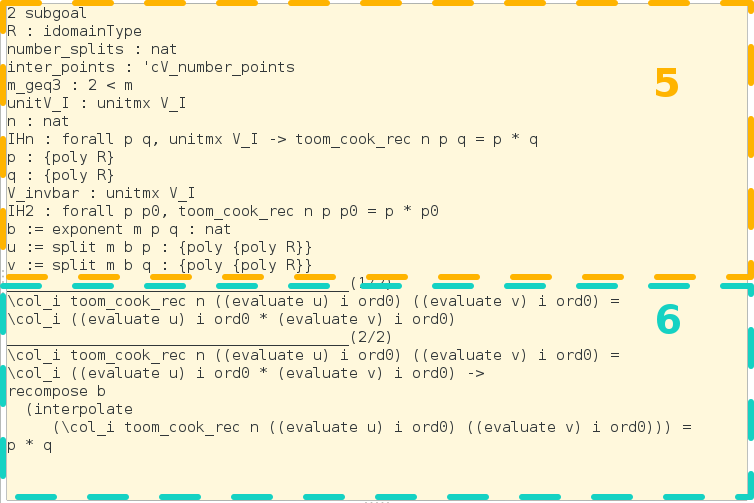
\includegraphics[width=150mm]{images/Kontext}
  \caption[Fönster för kontext och mål]
   {Textfönster för kontext och mål. Figuren visar en förstoring av ruta 2 i
    figur 4.1}
\end{figure}


\subsection{Evaluering av kod}
\coq är uppbyggt av satser där varje sats avslutas med en punkt. Koden
evalueras sedan en sats i taget och de delar av koden som har blivit evaluerade
markeras med en grön färg och det går inte längre att göra några ändringar i
dessa. Om man skulle vilja göra en ändring får man stega tillbaka
i programmet och göra ändringen.

\subsection{Bevis}
Det finns flera olika nyckelord för att starta ett bevis, bland annat
\C{Theorem} och \C{Lemma}. Det är ingen skillnad på vilket av dessa orden man
använder för att påbörja ett bevis utan de är bara till för att användaren ska
kunna gradera sina bevis. För enkelhetens skull kommer bara nyckelordet
\C{Lemma} användas i fortsättningen. Ett bevis i \coq är uppbyggt på följande
sätt

% verkar inte fungera med å i lstlisting
\begin{lstlisting}
Lemma bevisnamn : påstående som ska bevisas.
Proof.
  taktiker.
Qed.
\end{lstlisting}

Figur 4.3 visar ett exempel på ett bevis för att följande påstående är en
tautologi. En tautologi är en logisk sats som alltid är sant oberoende av
sanningsvärdena på hypoteserna.


\begin{figure}[H]
  \centering
  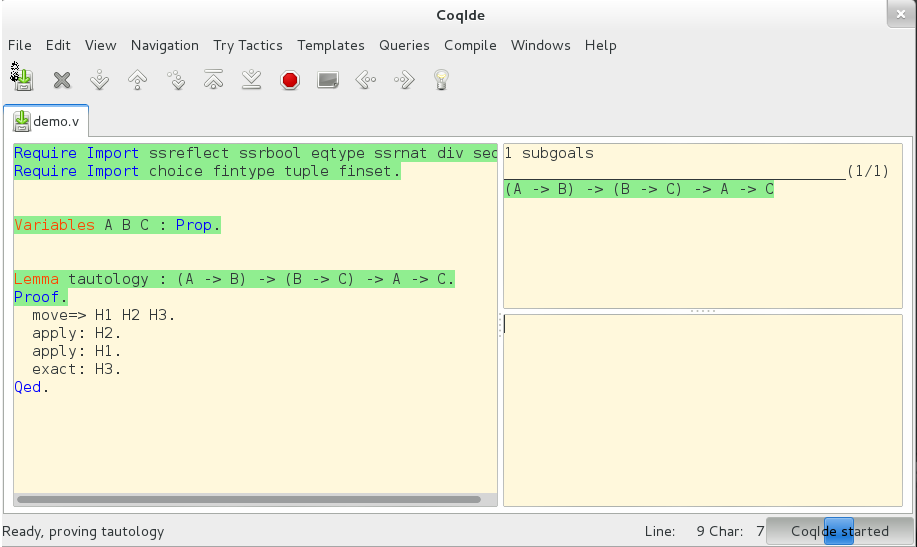
\includegraphics[width=100mm]{images/Proof_part1}
  \caption[Exempel på bevis i \coq]
   {Exempel på ett bevis för en tautologi i \coq}
\end{figure}

Figurerna 4.4 och 4.5 visar hur mål och kontext påverkas av de taktiker som
används.
Notera att de taktiker som har evaluerats blir grönmarkerade.
När alla mål är bevisade så talar man om att beviset är klart genom att skriva
\C{Qed} vilket översatt till svenska betyder "Vilket skulle bevisas".


\begin{figure}[H]
  \centering
  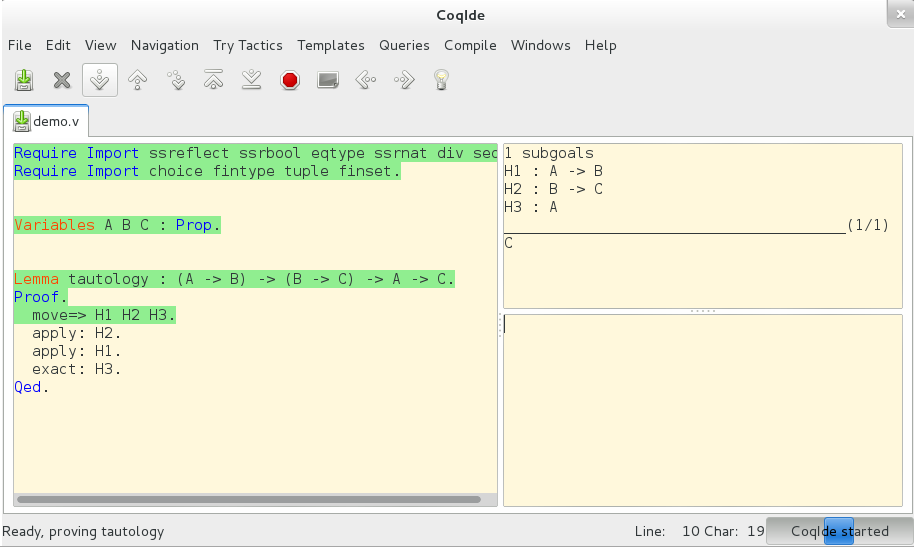
\includegraphics[width=150mm]{images/Proof_part2}
  \caption[Bevis i \coq Ide]
   {Vi har nu flyttat hypoteserna (A $rightarrow$ B), (B $\rightarrow$ C) och A
    från målet till kontexten och med taktiken \C{move}}
\end{figure}

\begin{figure}[H]
  \centering
  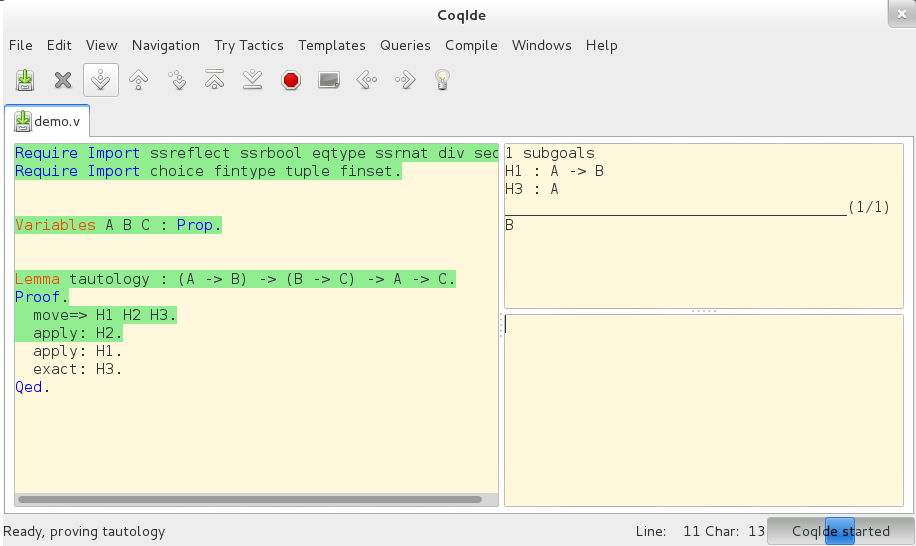
\includegraphics[width=150mm]{images/Proof_part3}
  \caption[Bevis i \coq Ide]
   {Vi har nu använt oss av Hypotesen (B \rightarrow C) och vi
    kan se att målet nu har ändrat sig från C till B}
\end{figure}


\subsection{Variabler och funktioner}

Det går att definiera variabler i \coq med nyckelordet \C{Varible}. När en
variabel deklareras på global nivå kan den sedan användas som parameter i bevis
och funktionsdefinitioner utan att behöva ange typen.

För att definiera funktioner och konstanter används nyckelordet
\C{Definition} som sedan sedan följs av funktions namn, parametrar och
funktionskropp.

\coq tillåter bara rekursion som är garanterad att avsluta. Det vill säga att
någon av parametrarna i det rekursiva kallet måste närma sig basfallet eller så
måste användaren ange ett bevis för att funktionen är garanterad att avsluta.
Så istället för att använda \C{Define} för att definiera en funktion måste
man använda \C{Fixpoint} istället. Det skulle till exempel inte gå att göra en
rekursiv funktion för Collatz problem i \coq.
Detta eftersom parametern bara
minskar om talet är jämt och det inte går att bevisa att basfallet alltid nås.
Collatz problem beskrivs i ekvation 4.1. En illustrativ beskrivning på hur detta
görs i återfinns i figur 4.6

\begin{equation}
T(n) = \left\{\begin{matrix} n/2, & \mbox{om }n\equiv0\mbox{ (mod 2)} \\ 3n+1,
                         & \mbox{om }n\equiv1\mbox{ (mod 2)} \end{matrix}\right.
\end{equation}





\subsection{Mönstermatchning}
Mönstermatchning i \coq påminner till stor del om \C{case} i Haskell.
Skillnaden är att istället för att skriva \C{case x of} som i Haskell så skrivs
\C{match x with} där x är namnet på variabeln som ska matchas i båda fallen.
I \coq måste även alla efterföljande rader utan den första börja med symbolen
$|$. Matchningssatsen måste även avslutas med \C{end}.

\begin{figure}[H]
  \centering
  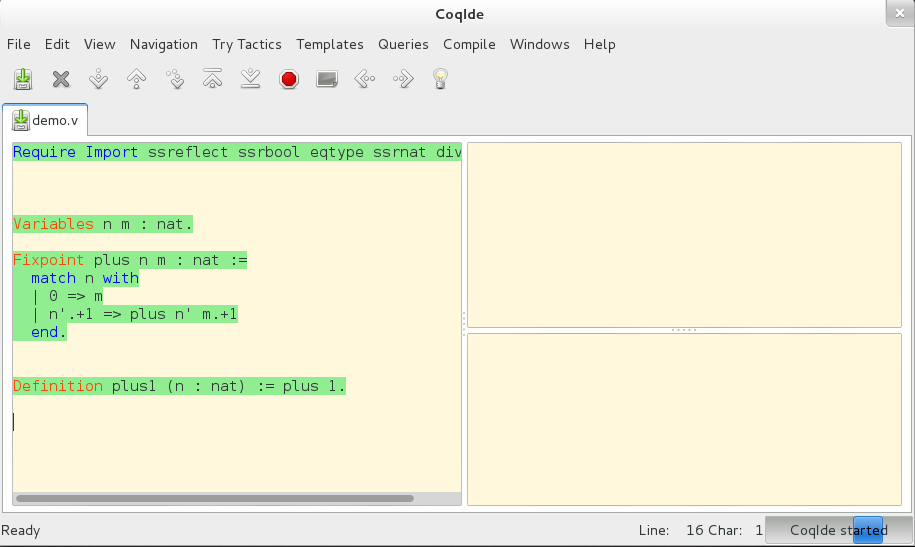
\includegraphics[width=150mm]{images/Variables_and_Functions}
  \caption[Variabler och funktioner]
   {Exempel på hur variabler och funktioner definieras i \coq}
\end{figure}
